
\documentclass[border=10pt, 12pt]{standalone}
\usepackage[svgnames]{xcolor}
\usepackage{amsmath}
\usepackage{pgfplots}
\pgfplotsset{compat=newest}
\usepackage[sfdefault]{FiraSans}
\usepackage{FiraMono}
\renewcommand*\familydefault{\sfdefault}
\begin{document}
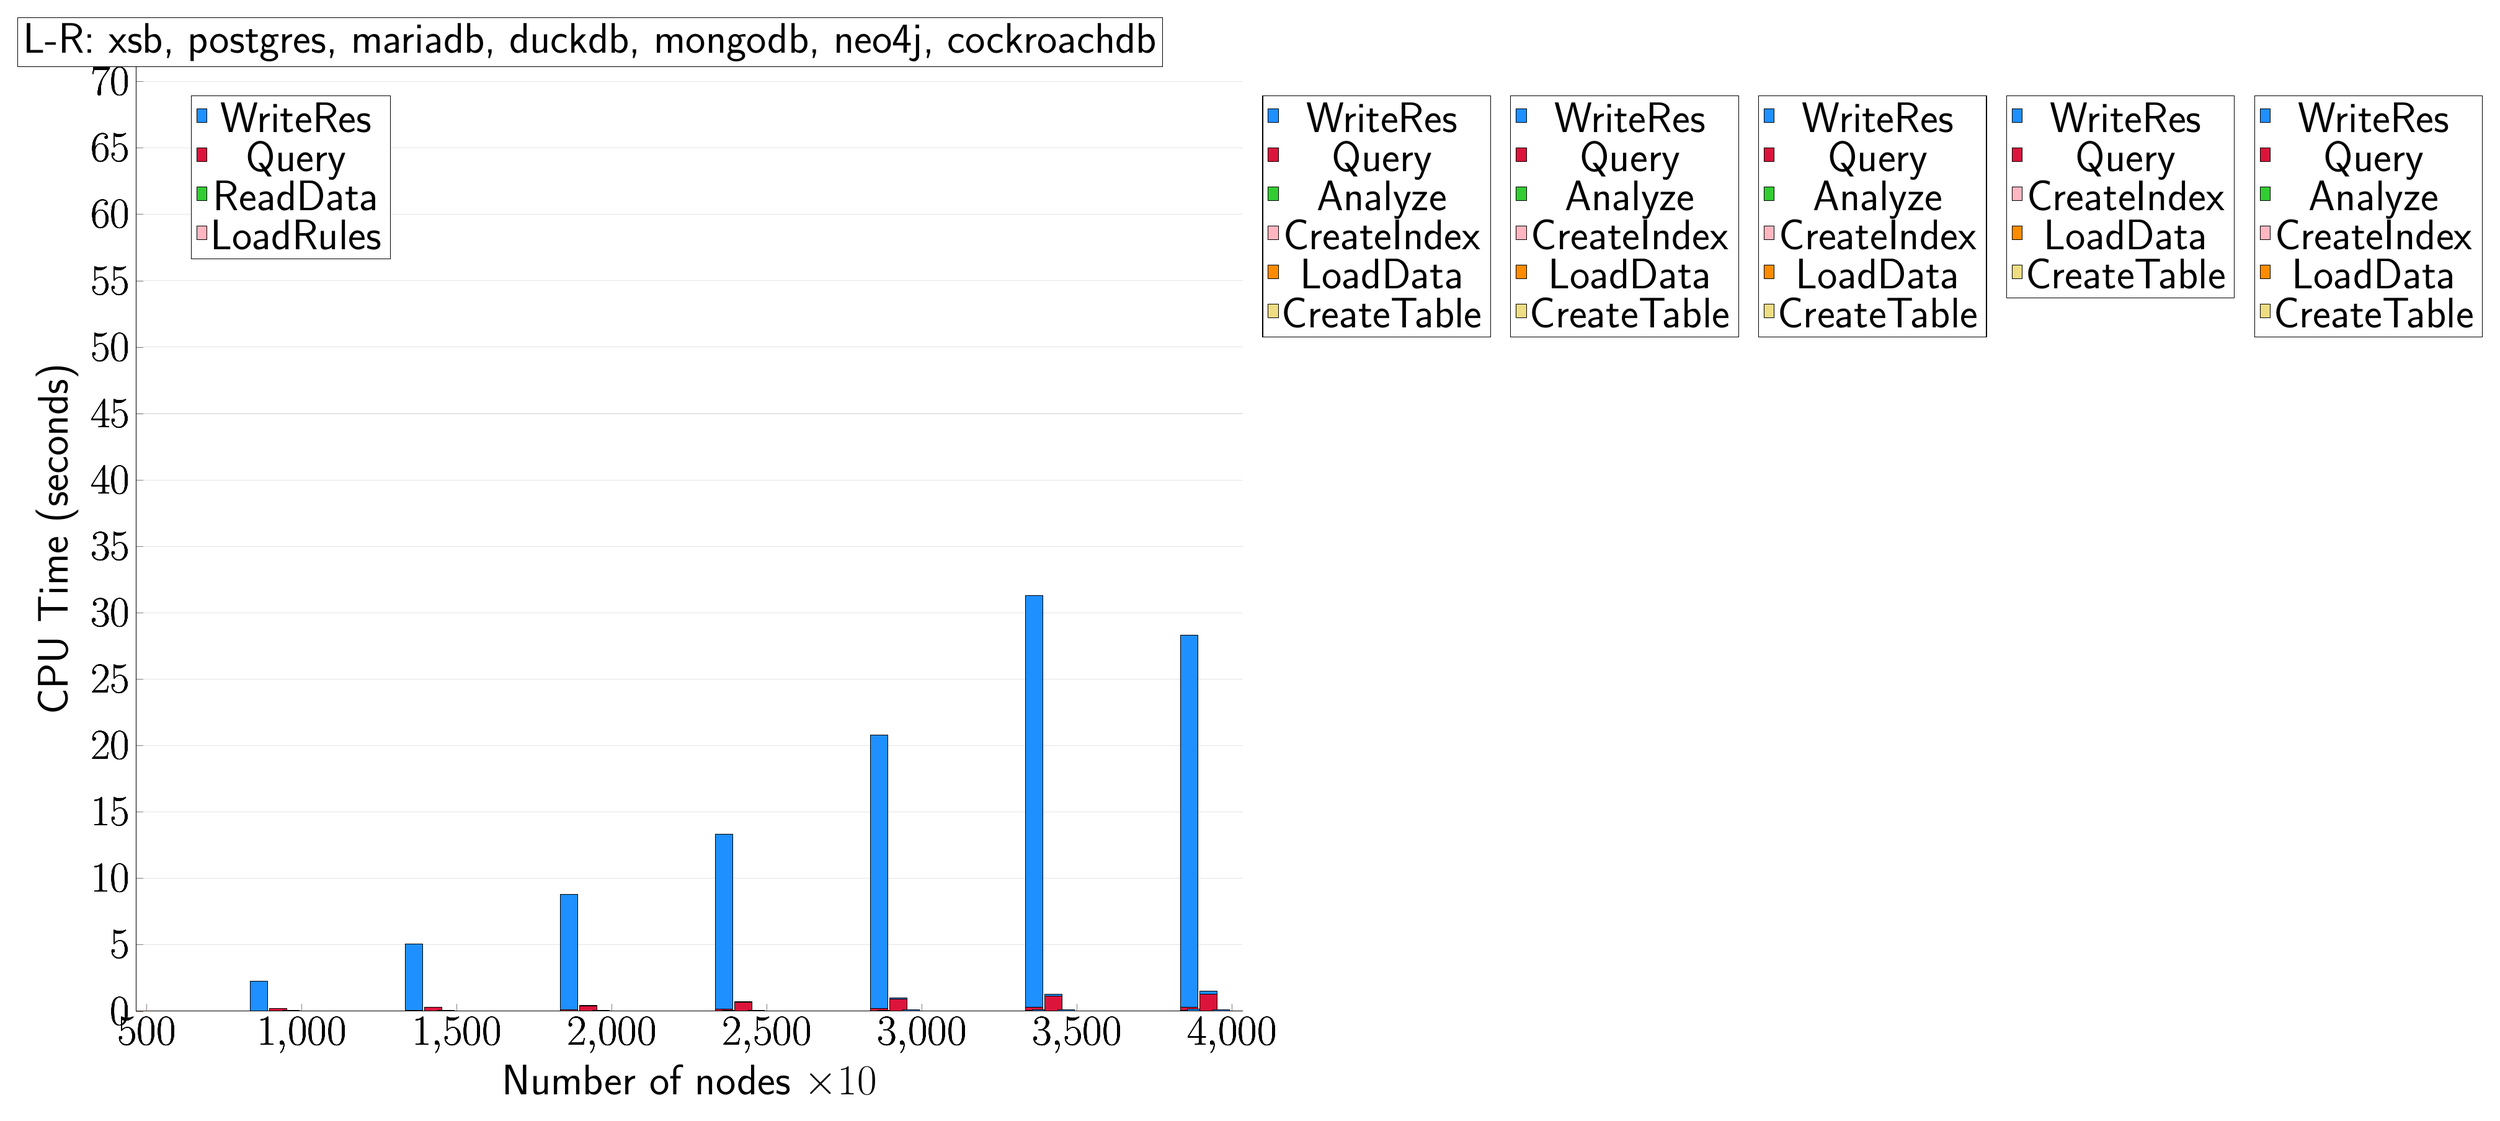
\begin{tikzpicture}
                        \begin{axis}[bar shift=-25pt, 
   ybar stacked,
   width=2\textwidth,
   bar width=0.35cm,
   ymajorgrids, tick align=inside,
   major grid style={draw=gray!20},
   xtick=data,
   ymin=0, ymax=71.079008658727,
   axis x line*=bottom,
   axis y line*=left,
   enlarge x limits=0.01,
   legend style={
       at={(0.23, 0.97)},
       anchor=north east,
       legend columns=1,
       font=\Huge,
   },
   ylabel={CPU Time (seconds)},
   xlabel={Number of nodes $\times 10$},
   label style={font=\Huge},
   tick label style={font=\Huge},
]
\addlegendimage{fill=DodgerBlue, draw=black, line width=0.2pt}
\addlegendentry{WriteRes}
\addlegendimage{fill=Crimson, draw=black, line width=0.2pt}
\addlegendentry{Query}
\addlegendimage{fill=LimeGreen, draw=black, line width=0.2pt}
\addlegendentry{ReadData}
\addlegendimage{fill=LightPink, draw=black, line width=0.2pt}
\addlegendentry{LoadRules}
\addplot +[fill=LightPink, draw=black, line width=0.2pt] coordinates {
(500, 0.0049440000000000005)
(1000, 0.004467666666666673)
(1500, 0.0033053333333333303)
(2000, 0.004451666666666664)
(2500, 0.004563)
(3000, 0.0044863333333333335)
(3500, 0.004998333333333337)
(4000, 0.0037359999999999997)
};
\addplot +[fill=LimeGreen, draw=black, line width=0.2pt] coordinates {
(500, 0.010025999999999998)
(1000, 0.015916666666666666)
(1500, 0.023359)
(2000, 0.029436)
(2500, 0.03692566666666667)
(3000, 0.04203833333333334)
(3500, 0.055746)
(4000, 0.04949633333333334)
};
\addplot +[fill=Crimson, draw=black, line width=0.2pt] coordinates {
(500, 0.003293333333333337)
(1000, 0.014888666666666666)
(1500, 0.03638333333333333)
(2000, 0.07140866666666668)
(2500, 0.11055366666666666)
(3000, 0.1566753333333333)
(3500, 0.25434066666666666)
(4000, 0.261251)
};
\addplot +[fill=DodgerBlue, draw=black, line width=0.2pt] coordinates {
(500, 0.6094946666666666)
(1000, 2.214624)
(1500, 5.005539)
(2000, 8.701642000000001)
(2500, 13.194564666666666)
(3000, 20.590858333333333)
(3500, 31.00154466666667)
(4000, 28.023601)
};
\end{axis}

\begin{axis}[bar shift=-21.3pt, 
   ybar stacked,
   width=2\textwidth,
   bar width=0.35cm,
   ymajorgrids, tick align=inside,
   major grid style={draw=none},
   xtick=data,
   ymin=0, ymax=71.079008658727,
   axis x line*=none,
   axis y line*=none,
   enlarge x limits=0.01,
   legend style={
       at={(1.224, 0.97)},
       anchor=north east,
       legend columns=1,
       font=\Huge,
   },
   label style={font=\Huge},
   tick label style={font=\Huge},
]
\addlegendimage{fill=DodgerBlue, draw=black, line width=0.2pt}
\addlegendentry{WriteRes}
\addlegendimage{fill=Crimson, draw=black, line width=0.2pt}
\addlegendentry{Query}
\addlegendimage{fill=LimeGreen, draw=black, line width=0.2pt}
\addlegendentry{Analyze}
\addlegendimage{fill=LightPink, draw=black, line width=0.2pt}
\addlegendentry{CreateIndex}
\addlegendimage{fill=DarkOrange, draw=black, line width=0.2pt}
\addlegendentry{LoadData}
\addlegendimage{fill=LightGoldenrod, draw=black, line width=0.2pt}
\addlegendentry{CreateTable}
\addplot +[fill=LightGoldenrod, draw=black, line width=0.2pt] coordinates {
(500, 0.0)
(1000, 0.0)
(1500, 0.0)
(2000, 0.0)
(2500, 0.0)
(3000, 0.0)
(3500, 0.0)
(4000, 0.0)
};
\addplot +[fill=DarkOrange, draw=black, line width=0.2pt] coordinates {
(500, 0.0)
(1000, 0.0)
(1500, 0.0)
(2000, 0.0)
(2500, 0.0)
(3000, 0.0)
(3500, 0.0)
(4000, 0.0)
};
\addplot +[fill=LightPink, draw=black, line width=0.2pt] coordinates {
(500, 0.0)
(1000, 0.0)
(1500, 0.0)
(2000, 0.0)
(2500, 0.006666666666666668)
(3000, 0.0)
(3500, 0.0)
(4000, 0.0)
};
\addplot +[fill=LimeGreen, draw=black, line width=0.2pt] coordinates {
(500, 0.0)
(1000, 0.0)
(1500, 0.0)
(2000, 0.0)
(2500, 0.0)
(3000, 0.0)
(3500, 0.0066666666666666515)
(4000, 0.0)
};
\addplot +[fill=Crimson, draw=black, line width=0.2pt] coordinates {
(500, 0.0)
(1000, 0.0)
(1500, 0.0)
(2000, 0.0)
(2500, 0.0)
(3000, 0.0)
(3500, 0.0)
(4000, 0.0)
};
\addplot +[fill=DodgerBlue, draw=black, line width=0.2pt] coordinates {
(500, 0.0)
(1000, 0.00999999999999999)
(1500, 0.019999999999999997)
(2000, 0.04666666666666667)
(2500, 0.05666666666666665)
(3000, 0.08333333333333333)
(3500, 0.10666666666666669)
(4000, 0.17666666666666667)
};
\end{axis}

\begin{axis}[bar shift=-17.6pt, 
   ybar stacked,
   width=2\textwidth,
   bar width=0.35cm,
   ymajorgrids, tick align=inside,
   major grid style={draw=none},
   xtick=data,
   ymin=0, ymax=71.079008658727,
   axis x line*=none,
   axis y line*=none,
   enlarge x limits=0.01,
   legend style={
       at={(1.448, 0.97)},
       anchor=north east,
       legend columns=1,
       font=\Huge,
   },
   label style={font=\Huge},
   tick label style={font=\Huge},
]
\addlegendimage{fill=DodgerBlue, draw=black, line width=0.2pt}
\addlegendentry{WriteRes}
\addlegendimage{fill=Crimson, draw=black, line width=0.2pt}
\addlegendentry{Query}
\addlegendimage{fill=LimeGreen, draw=black, line width=0.2pt}
\addlegendentry{Analyze}
\addlegendimage{fill=LightPink, draw=black, line width=0.2pt}
\addlegendentry{CreateIndex}
\addlegendimage{fill=DarkOrange, draw=black, line width=0.2pt}
\addlegendentry{LoadData}
\addlegendimage{fill=LightGoldenrod, draw=black, line width=0.2pt}
\addlegendentry{CreateTable}
\addplot +[fill=LightGoldenrod, draw=black, line width=0.2pt] coordinates {
(500, 0.0)
(1000, 0.0)
(1500, 0.0)
(2000, 0.0)
(2500, 0.0)
(3000, 0.0)
(3500, 0.0)
(4000, 0.0)
};
\addplot +[fill=DarkOrange, draw=black, line width=0.2pt] coordinates {
(500, 0.0)
(1000, 0.0)
(1500, 0.0)
(2000, 0.0)
(2500, 0.0)
(3000, 0.0)
(3500, 0.0)
(4000, 0.0)
};
\addplot +[fill=LightPink, draw=black, line width=0.2pt] coordinates {
(500, 0.0)
(1000, 0.010000000000000004)
(1500, 0.0)
(2000, 0.0)
(2500, 0.0)
(3000, 0.0)
(3500, 0.0)
(4000, 0.0)
};
\addplot +[fill=LimeGreen, draw=black, line width=0.2pt] coordinates {
(500, 0.0)
(1000, 0.0)
(1500, 0.0)
(2000, 0.0)
(2500, 0.0)
(3000, 0.0)
(3500, 0.0)
(4000, 0.0)
};
\addplot +[fill=Crimson, draw=black, line width=0.2pt] coordinates {
(500, 0.0)
(1000, 0.0)
(1500, 0.006666666666666669)
(2000, 0.0)
(2500, 0.0)
(3000, 0.0)
(3500, 0.0)
(4000, 0.0)
};
\addplot +[fill=DodgerBlue, draw=black, line width=0.2pt] coordinates {
(500, 0.0)
(1000, 0.0)
(1500, 0.0)
(2000, 0.0)
(2500, 0.0)
(3000, 0.0)
(3500, 0.0)
(4000, 0.0)
};
\end{axis}

\begin{axis}[bar shift=-13.899999999999999pt, 
   ybar stacked,
   width=2\textwidth,
   bar width=0.35cm,
   ymajorgrids, tick align=inside,
   major grid style={draw=none},
   xtick=data,
   ymin=0, ymax=71.079008658727,
   axis x line*=none,
   axis y line*=none,
   enlarge x limits=0.01,
   legend style={
       at={(1.6720000000000002, 0.97)},
       anchor=north east,
       legend columns=1,
       font=\Huge,
   },
   label style={font=\Huge},
   tick label style={font=\Huge},
]
\addlegendimage{fill=DodgerBlue, draw=black, line width=0.2pt}
\addlegendentry{WriteRes}
\addlegendimage{fill=Crimson, draw=black, line width=0.2pt}
\addlegendentry{Query}
\addlegendimage{fill=LimeGreen, draw=black, line width=0.2pt}
\addlegendentry{Analyze}
\addlegendimage{fill=LightPink, draw=black, line width=0.2pt}
\addlegendentry{CreateIndex}
\addlegendimage{fill=DarkOrange, draw=black, line width=0.2pt}
\addlegendentry{LoadData}
\addlegendimage{fill=LightGoldenrod, draw=black, line width=0.2pt}
\addlegendentry{CreateTable}
\addplot +[fill=LightGoldenrod, draw=black, line width=0.2pt] coordinates {
(500, 0.0)
(1000, 0.0)
(1500, 0.0)
(2000, 0.0066666666666666706)
(2500, 0.0)
(3000, 0.003333333333333332)
(3500, 0.0)
(4000, 0.0)
};
\addplot +[fill=DarkOrange, draw=black, line width=0.2pt] coordinates {
(500, 0.003333333333333318)
(1000, 0.003333333333333336)
(1500, 0.003333333333333336)
(2000, 0.003333333333333336)
(2500, 0.006666666666666669)
(3000, 0.013333333333333343)
(3500, 0.010000000000000005)
(4000, 0.009999999999999972)
};
\addplot +[fill=LightPink, draw=black, line width=0.2pt] coordinates {
(500, 0.003333333333333336)
(1000, 0.003333333333333336)
(1500, 0.0)
(2000, 0.003333333333333318)
(2500, 0.003333333333333336)
(3000, 0.0)
(3500, 0.0)
(4000, 0.0)
};
\addplot +[fill=LimeGreen, draw=black, line width=0.2pt] coordinates {
(500, 0.0)
(1000, 0.0)
(1500, 0.0)
(2000, 0.0)
(2500, 0.0)
(3000, 0.003333333333333337)
(3500, 0.003333333333333318)
(4000, 0.0)
};
\addplot +[fill=Crimson, draw=black, line width=0.2pt] coordinates {
(500, 0.08333333333333333)
(1000, 0.18999999999999997)
(1500, 0.29333333333333333)
(2000, 0.4033333333333333)
(2500, 0.6533333333333332)
(3000, 0.91)
(3500, 1.13)
(4000, 1.2833333333333334)
};
\addplot +[fill=DodgerBlue, draw=black, line width=0.2pt] coordinates {
(500, 0.0)
(1000, 0.010000000000000009)
(1500, 0.02333333333333334)
(2000, 0.0366666666666667)
(2500, 0.06333333333333337)
(3000, 0.09666666666666675)
(3500, 0.12333333333333336)
(4000, 0.2166666666666666)
};
\end{axis}

\begin{axis}[bar shift=-6.5pt, 
   ybar stacked,
   width=2\textwidth,
   bar width=0.35cm,
   ymajorgrids, tick align=inside,
   major grid style={draw=none},
   xtick=data,
   ymin=0, ymax=71.079008658727,
   axis x line*=none,
   axis y line*=none,
   enlarge x limits=0.01,
   legend style={
       at={(1.896, 0.97)},
       anchor=north east,
       legend columns=1,
       font=\Huge,
   },
   label style={font=\Huge},
   tick label style={font=\Huge},
]
\addlegendimage{fill=DodgerBlue, draw=black, line width=0.2pt}
\addlegendentry{WriteRes}
\addlegendimage{fill=Crimson, draw=black, line width=0.2pt}
\addlegendentry{Query}
\addlegendimage{fill=LightPink, draw=black, line width=0.2pt}
\addlegendentry{CreateIndex}
\addlegendimage{fill=DarkOrange, draw=black, line width=0.2pt}
\addlegendentry{LoadData}
\addlegendimage{fill=LightGoldenrod, draw=black, line width=0.2pt}
\addlegendentry{CreateTable}
\addplot +[fill=LightGoldenrod, draw=black, line width=0.2pt] coordinates {
(500, 0.0)
(1000, 0.010000000000000004)
(1500, 0.010000000000000005)
(2000, 0.0033333333333333375)
(2500, 0.010000000000000009)
(3000, 0.003333333333333337)
(3500, 0.0)
(4000, 0.006666666666666654)
};
\addplot +[fill=DarkOrange, draw=black, line width=0.2pt] coordinates {
(500, 0.006666666666666675)
(1000, 0.0)
(1500, 0.0)
(2000, 0.0)
(2500, 0.0)
(3000, 0.0)
(3500, 0.003333333333333336)
(4000, 0.0)
};
\addplot +[fill=LightPink, draw=black, line width=0.2pt] coordinates {
(500, 0.0033333333333333184)
(1000, 0.0)
(1500, 0.0)
(2000, 0.010000000000000004)
(2500, 0.0)
(3000, 0.003333333333333318)
(3500, 0.003333333333333337)
(4000, 0.003333333333333336)
};
\addplot +[fill=Crimson, draw=black, line width=0.2pt] coordinates {
(500, 0.0)
(1000, 0.006666666666666674)
(1500, 0.003333333333333332)
(2000, 0.0)
(2500, 0.0)
(3000, 0.00666666666666665)
(3500, 0.0)
(4000, 0.0)
};
\addplot +[fill=DodgerBlue, draw=black, line width=0.2pt] coordinates {
(500, 0.01333333333333333)
(1000, 0.03666666666666663)
(1500, 0.05333333333333332)
(2000, 0.06)
(2500, 0.06999999999999999)
(3000, 0.08666666666666667)
(3500, 0.11000000000000003)
(4000, 0.11000000000000003)
};
\end{axis}

\begin{axis}[bar shift=-2.799999999999997pt, 
   ybar stacked,
   width=2\textwidth,
   bar width=0.35cm,
   ymajorgrids, tick align=inside,
   major grid style={draw=none},
   xtick=data,
   ymin=0, ymax=71.079008658727,
   axis x line*=none,
   axis y line*=none,
   enlarge x limits=0.01,
   legend style={
       at={(2.12, 0.97)},
       anchor=north east,
       legend columns=1,
       font=\Huge,
   },
   label style={font=\Huge},
   tick label style={font=\Huge},
]
\addlegendimage{fill=DodgerBlue, draw=black, line width=0.2pt}
\addlegendentry{WriteRes}
\addlegendimage{fill=Crimson, draw=black, line width=0.2pt}
\addlegendentry{Query}
\addlegendimage{fill=LimeGreen, draw=black, line width=0.2pt}
\addlegendentry{Analyze}
\addlegendimage{fill=LightPink, draw=black, line width=0.2pt}
\addlegendentry{CreateIndex}
\addlegendimage{fill=DarkOrange, draw=black, line width=0.2pt}
\addlegendentry{LoadData}
\addlegendimage{fill=LightGoldenrod, draw=black, line width=0.2pt}
\addlegendentry{CreateTable}
\addplot +[fill=LightGoldenrod, draw=black, line width=0.2pt] coordinates {
(500, 0.0)
(1000, 0.0)
(1500, 0.0)
(2000, 0.0)
(2500, 0.0)
(3000, 0.0)
(3500, 0.0)
(4000, 0.0)
};
\addplot +[fill=DarkOrange, draw=black, line width=0.2pt] coordinates {
(500, 0.003333333333333336)
(1000, 0.0)
(1500, 0.0)
(2000, 0.0)
(2500, 0.0)
(3000, 0.0)
(3500, 0.0033333333333333327)
(4000, 0.0)
};
\addplot +[fill=LightPink, draw=black, line width=0.2pt] coordinates {
(500, 0.0)
(1000, 0.0)
(1500, 0.0)
(2000, 0.010000000000000007)
(2500, 0.0)
(3000, 0.0)
(3500, 0.0)
(4000, 0.0)
};
\addplot +[fill=LimeGreen, draw=black, line width=0.2pt] coordinates {
(500, 0.0)
(1000, 0.0)
(1500, 0.0)
(2000, 0.0)
(2500, 0.0)
(3000, 0.0)
(3500, 0.0)
(4000, 0.0)
};
\addplot +[fill=Crimson, draw=black, line width=0.2pt] coordinates {
(500, 0.0)
(1000, 0.0)
(1500, 0.0)
(2000, 0.0)
(2500, 0.0)
(3000, 0.0)
(3500, 0.0)
(4000, 0.0)
};
\addplot +[fill=DodgerBlue, draw=black, line width=0.2pt] coordinates {
(500, 0.0)
(1000, 0.0)
(1500, 0.0)
(2000, 0.0)
(2500, 0.0)
(3000, 0.0)
(3500, 0.0)
(4000, 0.0)
};
\end{axis}


\node[anchor=south, draw, fill=white] at (rel axis cs:0.42,1) {\Huge L-R: xsb, postgres, mariadb, duckdb, mongodb, neo4j, cockroachdb};
\end{tikzpicture}
\end{document}
                    